\documentclass{article}
\usepackage[a4paper, total={6in, 8in}]{geometry}
\usepackage{algorithm}
\usepackage{algpseudocode}
\usepackage{float}
\usepackage{hyperref}
\usepackage{graphicx}
\graphicspath{ {images/} }
\usepackage{tcolorbox}
\usepackage[utf8]{inputenc}
\usepackage[english]{babel}
\usepackage{amsthm}
\theoremstyle{definition}
\newtheorem{definition}{Definition}[section]
\usepackage{forest}

\usepackage{listings}
\usepackage{color}
\usepackage{multirow}
\usepackage{tabularx}
\definecolor{folderbg}{RGB}{124,166,198}
\definecolor{folderborder}{RGB}{110,144,169}
\definecolor{dkgreen}{rgb}{0,0.6,0}
\definecolor{gray}{rgb}{0.5,0.5,0.5}
\definecolor{mauve}{rgb}{0.58,0,0.82}
\definecolor{lbcolor}{rgb}{0.9,0.9,0.9}

\def\Size{4pt}
\tikzset{
  folder/.pic={
    \filldraw[draw=folderborder,top color=folderbg!50,bottom color=folderbg]
      (-1.05*\Size,0.2\Size+5pt) rectangle ++(.75*\Size,-0.2\Size-5pt);
    \filldraw[draw=folderborder,top color=folderbg!50,bottom color=folderbg]
      (-1.15*\Size,-\Size) rectangle (1.15*\Size,\Size);
  }
}

\lstset{
tabsize=4,
basicstyle=\ttfamily,
backgroundcolor=\color{lbcolor},
showstringspaces=false
}
% \lstset{frame=tb,
%   language=Java,
%   aboveskip=3mm,
%   belowskip=3mm,
%   showstringspaces=false,
%   columns=flexible,
%   basicstyle={\small\ttfamily},
%   numbers=none,
%   numberstyle=\tiny\color{gray},
%   keywordstyle=\color{blue},
%   commentstyle=\color{dkgreen},
%   stringstyle=\color{mauve},
%   breaklines=true,
%   breakatwhitespace=true,
%   tabsize=3
% }

\newcommand{\green}[1]{\colorbox{green!30}{#1}}
\newcommand{\blue}[1]{\colorbox{blue!30}{#1}}
\newcommand{\tpurple}[1]{\textcolor{purple!30}{#1}}

\begin{document}

\begin{titlepage}
	\newcommand{\HRule}{\rule{\linewidth}{0.5mm}}
	\center % Centre everything on the page
	\textsc{\LARGE Iowa State University}\\[1.5cm]
	\HRule\\[0.4cm]
	{\huge\bfseries R2U2 System Documentation}\\[0.4cm]
	\HRule\\[1.5cm]
	\vfill\vfill\vfill
	{\large\today}
	\vfill
\end{titlepage}


\tableofcontents
\clearpage

\section{Nomenclature}
All the informaiton requried to use R2U2 is called the \emph{configuration}.
A R2U2 configuration incudes \emph{design-time configuration} and \emph{runtime configuration}.
The design time configuration provides additional informtion to an \emph{implmentation} of the R2U2 engine to create a \emph{unit}.
A depoloyed unit can monitor different specificaitons at runtime by loading different runtime configurations.

\begin{description}
    \item[R2U2 Configuration]{A combination of the requried design time and runtime infoamtion to deploy R2U2}
    \item[Design-time Configuration]{Settings for tailoring the R2U2 engine for a deployment, e.g. compiler settings, FPGA parameters, etc.}
    \item[Runtime Configuration]{Specificaitons to be monitored by R2U2}
    \item[Implmentation]{The source of an R2U2 engine, written in a programming or hardware description language}
    \item[Unit]{The result of configuring an R2U2 implmentation, executable bytecode or sythezized hardware}
    \item[Deployment]{One or many R2U2 units targeted at, and configured to provide system health monitoring for, a system.}
\end{description}
\clearpage

\section{R2U2 Software (C)}

\subsection{Process Overflow}
Figure \ref{fig:c_flow} shows the procedure of running the R2U2 C version by the user. From the high level, the user need to specify the MLTL formulas first. The formula will be converted into 1) binary instruction file; 2) SCQ size assignment file; 3) intervals for each temporal instruction. The user should also prepare the sensor trace file (*.trc) for verification.
\begin{figure}[H]
  \includegraphics[scale=0.50]{fig/r2u2_c_flow.pdf}
  \caption{Deploying steps of R2U2 C. Blocks marked in green are the files required for the program execution. The yellow blocks tells the dependency of the tool scripts that handle the conversion.}
  \label{fig:c_flow}
\end{figure}

\subsection{R2U2 C Operation Modes and Trace Input Format}
There are two operation modes for R2U2 C: 1) Offline mode (regression test) 2) Online mode (embedded application).

To select the operation mode, comment/uncomment the line: \\
\colorbox{blue!30}{"\#define ONLINE\_MODE"} in \colorbox{gray!30}{r2u2/R2U2\_SW/R2U2\_C/src/R2U2.c}\\
and recompile the C program. Under different modes, the trace input is different (check Table \ref{tab:c_trace}).

\begin{table}[ht]
  \caption{Format and content of trace file}
  \label{tab:c_trace}
  \begin{center}
  \begin{tabular}{c|cccc|cccc}
      \hline
      Mode&\multicolumn{4}{c|}{Offline Mode}&\multicolumn{4}{c}{Online Mode}\\
      \cline{1-9}
      \multirow{1}{*}{Column Information}&sensor 0&sensor 1&sensor 2&\multicolumn{1}{c|}{...}&Command&sensor 0&sensor 1&...\\
      \hline
      \multirow{3}{*}{*.trc File Content}& 1.0 & 2.0 & 1.2 &...& -1 & 1.0 & 2.0 &...\\
      & 0.8 & 1.2 & 1.3 &...  & & & \\
      & 0.5 & 1.1 & 1.2 &... & & &  \\
      &...& & & ...& & & \\
      \hline
  \end{tabular}
  \end{center}
  \label{tab:multicol}
  \end{table}
Under the online mode, the command is included into the *.trc file. The trace file should be updated at each time stamp. In order to specify the behavior for R2U2, we use the first column in the trace file as the command to R2U2. The \textbf{command} variable can only be integers. If command=-2, R2U2 will terminate. If command=-1, R2U2 will reset the buffer and prepare for the new round of execution. The positive number of command represents the timestamp of the sensor value. Users should guarantee the timestamp will increase 1 by 1 starting from 0. Table \ref{tab:c_command_trace} summarizes the meaning of the \textbf{command} variable.
\begin{table}[h]
  \begin{tabularx}{\textwidth}{ |l|X| } 
   \hline
   Command Value & Description \\ 
   \hline
   -2 & Terminate the current execution. \\ 
   \hline
   -1 & Reset the instruction/data etc. buffer to restart the RV. Users must set command to -1 as the RV starts signal or the RV engine will not start.\\ 
   \hline
   i (Positive Integers) & Represent the sensor signal at time stamp i. The i should increase by 1 each time, starting from 0. (Increasing i tells the RV engine that new sensor value is coming.)\\
   \hline
   others & Unspecified\\
   \hline
  \end{tabularx}
  \caption{Meaning of `command' variable in *.trc file.}
  \label{tab:c_command_trace}
\end{table}


\subsection{Atomic Conversion Function}
% The sensor data in the *.trc file is the \colorbox{gray!30}{r2u2/R2U2\_SW/R2U2\_C/inputs/} folder.
Users need to manually specify the atomic conversion function. The function is specified in file: \\
\colorbox{gray!30}{r2u2/R2U2\_SW/R2U2\_C/src/AT/at\_conversion.c}. \\
Below is an example of the conversion function:
\begin{lstlisting}[language=C]
void at_checkers_update(const r2u2_input_data_t *r2u2_input_data){
	for (int i=0; i< N_ATOMICS; i++){
		atomics_vector[i] = AT_COMP((r2u2_input_data[i]), > , 0.5);
	}
}
\end{lstlisting}
,where \colorbox{blue!30}{atomics\_vector[i]} corresponds to atomic $a_i$ in the MLTL formula. \colorbox{blue!30}{r2u2\_input\_data[i]} corresponds to \textit{sensor i} in the trace file.
Uses can borrow some math marcos in \colorbox{gray!30}{at\_checkers.h} under the same folders or write their own math functions. 



\subsection{Command Line R2U2 C Execution}

\begin{table}[ht]
  \caption{Software dependency and the prerequisites}
  \label{tab:c_trace}
  \begin{center}
  \begin{tabular}{c|c}
      \hline
      \multirow{2}{*}{MLTL Compiler}& version $\geq$ python 3.0\\
      \cline{2-2}
      & ply; (pip install ply)\\
      \hline
      \multirow{2}{*}{R2U2 C}& pkg-config; (sudo apt install pkg-config)\\
      \cline{2-2}
      &  fftw3; (sudo apt-get install libfftw3-dev libfftw3-doc)\\
      \hline
  \end{tabular}
  \end{center}
  \label{tab:multicol}
  \end{table}

After determining the running mode and the trace file, now we can build the C project and check the execution output. Here is the steps for deploying the R2U2 C:
\begin{enumerate}
  \item Compile the C program:
    \begin{itemize}
      \item Navigate to the src folder
      \begin{lstlisting}[language=Bash]
      cd r2u2/R2U2-SW/R2U2_C/src/
      \end{lstlisting}
      \item Call MakeFile to compile
      \begin{lstlisting}[language=Bash]
      make
      \end{lstlisting}
    \end{itemize}

  \item Generate configuration files:
    \begin{itemize}
      \item Navigate to the tools/ folder:
      \begin{lstlisting}[language=Bash]
      cd r2u2/tools/
      \end{lstlisting}
      \item Convert MLTL formula to assembly:
      \begin{lstlisting}[language=Bash]
      python Compiler/main.py [MLTL formula]
      \end{lstlisting}
      This command will generate \textbf{tmp.ftasm} and \textbf{tmp.ftscq} configuration files.
      For the syntax of MLTL formula, refer to ??. (Note: special symbol (e.g., \&,$($,$)$,\textit{space}, etc.) should put a `\textbackslash' in the front).
      \item Convert assembly to binary text:
      \begin{lstlisting}[language=Bash]
      %#cat tmp.ftasm | python AssemblyToBinary/ftas.py tmp
      python AssemblyToBinary/ftas.py tmp.ftasm 4
      \end{lstlisting}
      This results the file \textbf{tmp.ftm} and \textbf{tmp.fti}.
    \end{itemize}

  \item Specify the trace file and start
  \begin{lstlisting}[language=Bash]
    bin/r2u2 [trace file *.trc]
  \end{lstlisting}
  If under online mode, then the user is in charge of updating the trace file at each time stamp.
\end{enumerate}

\clearpage

\clearpage

\section{R2U2 Software (Cpp)}
(Require C++11)

\subsection{Assembly Mode Configuration}
In main file MTL.cpp:
\begin{enumerate}
\item  Assign the sensor number, simulation time stamps;
\item  Link the sensor to the .log file;
\end{enumerate}
\begin{lstlisting}[language=C]
sensor[0]=new Event("./src/alt.log");
sensor[1]=new Event("./src/pitch.log");
\end{lstlisting}

In assembly code file test.ftasm:
\begin{enumerate}
\item Write the assembly code in test.ftasm
\item Specify the assembly code file
\end{enumerate}
\begin{lstlisting}[language=C]
string asm_file="./src/test.ftasm";
\end{lstlisting}

\subsection{MLTL Mode Configuration:}
In main file MTL.cpp:
\begin{enumerate}
\item Assign the sensor number, simulation time stamps;
\item Link the sensor to the .log file;
\item Write your MTL formula as a string in MTL.cpp. For MTL format, see Notes;
\end{enumerate}


\subsection{How to Run}
In terminal:
\begin{enumerate}
\item run setup.sh to compile the project
\begin{lstlisting}[language=Bash]
bash setup.sh
\end{lstlisting}
\item type ./Debug/MTL to running MTL
\begin{lstlisting}[language=Bash]
bash ./Debug/MTL
\end{lstlisting}
\end{enumerate}

Notes: Meaning the MTL String:
\begin{lstlisting}[language=C]
Algorithm 1: "!" = "NOT{}"
Algorithm 2: "G[2]" = "KEP[2]{}"
Algorithm 3: "&" = "AND{,}"
Algorithm 4: "G[2,5]" = "ALW[2,5]{}"
Algorithm 5: "F[1,2]" = "UNT[1,2]{,}"
\end{lstlisting}

\begin{lstlisting}[language=C]
string formula="NOT{S[0]}";
string formula="NOT{NOT{S[0]}}";
string formula="KEP[5]{S[1]}";
string formula="NOT{KEP[2]{NOT{S[1]}}}";
string formula="AND{KEP[2]{S[0]},S[1]}";
string formula="ALW[5,10]{S[1]}";
string formula="NOT{AND{ALW[5,10]{S[0]},KEP[2]{S[1]}}}";
string formula="AND{KEP[2]{NOT{NOT{S[0]}}},S[0]}";
string formula="AND{S[1],ALW[0,8]{S[0]}}";
string formula="AND{S[1],KEP[8]{S[0]}}";
string formula="AND{ALW[5,10]{S[0]},KEP[2]{S[1]}}";
string formula="KEP[2]{S[1]}";
string formula="AND{AND{S[0],S[1]},ALW[3,5]{S[0]}}";
\end{lstlisting}

\clearpage

\clearpage

\section{R2U2 Software (Python)(Requires python 3.X)}
The current python version only supports offline test. Python R2U2 is suitable for research purpose if you want to check how the SCQ works or the observer algorithm.
The python version code is located under the repository: \colorbox{gray!30}{r2u2/R2U2\_SW/R2U2\_PYTHON/}.
\subsection{Process Overflow}
\begin{figure}[H]
	\includegraphics[scale=0.50]{fig/r2u2_python_flow.pdf}
	\caption{Deploying steps of R2U2 Python.}
	\label{fig:python_flow}
\end{figure}

User can run the R2U2 python in terminal:
\begin{lstlisting}[language=Bash]
	python MLTL_main.py -m "$(cat [A])" -s [B] -o [C]
\end{lstlisting}
\begin{tcolorbox}
A: Assembly/MLTL Input File: Assembly code in a file or MLTL formula written in a file\\
B: Signal Trace File. Refer to Section \ref{sec:python_trace_format} for detail format. \\
C: Output File. The RV result will be written into the file. If user did not specify \textbf{-o} option, the output file will be default 'untitled.txt'.
\end{tcolorbox}
Or
\begin{lstlisting}[language=Bash]
	python MLTL_main.py -m [A] -s [B] -o [C]
\end{lstlisting}
\begin{tcolorbox}
A: MLTL formula (Take care of special symbol in command line)\\
B: Signal Trace File. Refer to Section \ref{sec:python_trace_format} for detail format. \\
C: Output File. The RV result will be written into the file. If user did not specify \textbf{-o} option, the output file will be default 'untitled.txt'.
\end{tcolorbox}


\subsection{Input Trace Format and Boolean Function}
\label{sec:python_trace_format}
Table \ref{tab:python_trace} shows the input format for the trace input file.
\begin{table}[ht]
	\caption{Format and content of trace file}
	\label{tab:python_trace}
	\begin{center}
	\begin{tabular}{c|cccc|cccc}
		\hline
		Mode&\multicolumn{4}{c|}{Atomic Input Format(0/1)}&\multicolumn{4}{c}{Sensor Input Format(floating)}\\
		\cline{1-9}
		\multirow{1}{*}{Column Information}&atomic 0&atomic 1&atomic 2&\multicolumn{1}{c|}{...}&sensor 0&sensor 1&sensor 2&...\\
		\hline
		\multirow{3}{*}{trace file content}& a0 & a1 & a2 &...& altitude & velocity & temp &...\\
		& 0 & 1 & 1 &...  & 1005& 32.7 &87 \\
		& 0 & 0 & 1 &... & 1010& -1.7 &87  \\
		&...& & & ...& ...&  & \\
		\hline
	\end{tabular}
	\end{center}
	\label{tab:multicol}
	\end{table}
In the trace input file, the first row is the trace name. After the first row, each line is the data in a seperate time stamp ranging from 0. E.g., the second row is data in time stamp 0, third row is data in time stamp 1. For each column (split by either space or comma), the first column data is signal trace 0. The second column data is signal trace 1 and so on. \\
Note that 1) For atomic input format, the atomic name should be consistent with the atomic name in MLTL specification; 2) For sensor Input, the sensor name should be consistent with the boolean function in \colorbox{gray!30}{r2u2/R2U2\_SW/R2U2\_PYTHON/ACOW/Traverse.py} function \colorbox{blue!30}{s2a(self,signal\_trace)}. The atomic map in the function should be consistent with the MLTL specification. Below is the example for function \colorbox{blue!30}{s2a(self,signal\_trace)}:
\begin{lstlisting}[language=Python]
def s2a(self,signal_trace):	
	atomic_map = {}
	s2d = {signal_name:i for i,signal_name in enumerate(self.trace_name)}

	##################################################################
	# For User: map boolean function to atomic
	atomic_map['a0'] = abs(s2d['altitude'])<0.04
	atomic_map['a1'] = abs(s2d['velocity'])<0.08
	atomic_map['a2'] = s2d['temp']>0.6
	##################################################################
	return atomic_map
\end{lstlisting}

\subsection{AST Optimization}
AST optimization only works in MLTL formula input. If you want to optimize the AST, change the input argument in function \colorbox{blue!30}{formula\_input()}. The following line of code in MTL\_main.py:
\begin{lstlisting}[language=Python]
	valid_node_set = formula_input(MLTL) # optimize
	valid_node_set = formula_input(MLTL,False) # unoptimize
\end{lstlisting}

\subsection{Model Checking (not used in R2U2)}
\subsubsection{Define Automata} \label{sec:aut}
You can specify the input as the automata.
\begin{lstlisting}[language=Python]
def define_automaton():
	a = automaton()
	#sg = StateGen(3,'s','a') # call function to autogenerate state for you
	a.INITIAL_STATE = 's2'
	a.DEST_STATE = 's3'
	#a.STATE, a.DELTA = sg.gen_aut()
	a.STATE = {
	's0':{'a0':0,'a1':0},
	's1':{'a0':0,'a1':1},
	's2':{'a0':1,'a1':0},
	's3':{'a0':1,'a1':1},
	}
	a.DELTA = {
	's0': {'s0','s1','s2','s3'},
	's1': {'s0','s1','s2','s3'},
	's2': {'s0','s1','s2','s3'},
	's3': {'s0','s1','s2','s3'},
	}
	print(a)
	return a
\end{lstlisting}

\subsubsection{Run Model Checking}
The tool supports model checking for a MLTL formula given the automata. User need to define the automata with initial state \textbf{INITIAL\_STATE} and desired end state \textbf{DEST\_STATE}.
\begin{lstlisting}[language=Python]
	a = define_automaton()
	a.init()
	valid_node_set = assembly_input(MLTL)
	solution = Search(a,valid_node_set,agent='DES')
\end{lstlisting}
\clearpage

\clearpage

\section{Run R2U2 in Vivado Simulation}
(Tested in Vivado 2017.02)
\subsection{Name of Binary Files:}
The HW simulator takes the binary assembly code as input. There are three binary files that are necessary to run the HW simulation:
\begin{itemize}
\item *.trc: Input signal at each time stamp;
\item *int: Intervals of certain operations;
\item *imem: Binary assembly code without interval.
\end{itemize}

\subsection{Steps to build the project:}
\begin{enumerate}
  \item In vivado command window, \textbf{cd} into the folder\\
  \textbf{/r2u2/R2U2\_HW/Hardware/hdl/ftMuMonitor/vivado}
  \item Click Tools$\rightarrow$ Run Tcl Script. Then Choose the .tcl file under current directory
  \item Rewrite the *.trc, *.int, *.imem to test different cases (Refer to \hyperlink{gb}{"How to generate binary file for the HW test" })
  \item The async result is shown in the file \textbf{async\_out.txt} under the folder\\
  \textbf{/r2u2/R2U2\_HW/Hardware/hdl/ftMuMonitor/vivado/FT\_Monitor/FT\_Monitor.sim/\\
  sim\_1/behav}
\end{enumerate}
\hypertarget{gb}{\subsection{How to generate binary file for the HW test:}}
\begin{enumerate}
	\item Write the assembly code in casestudy.ftasm under directory\\
 \textbf{r2u2/R2U2\_HW/Software/ftAssembler/}
	\item run \textbf{./convert.sh} under that folder. The script will call the python script to generate the binary file (*.imem, *.int). It will automatically copy these files into the vivado project.
	\item The input signal is called \textbf{atomic.trc} located under \\
\textbf{r2u2/R2U2\_HW/Hardware/hdl/ftMuMonitor/sim/testbench/}. Each signal is written into a column. The first signal is in column 0.
\end{enumerate}

\clearpage
\clearpage


\section{Running on the FPGA}
This section talks about how to generate required files and steps to run the demo. \\
Note: 1) The text mark with \colorbox{blue!30}{\hspace{0.5cm}} means the command typed in terminal.\\
2) The text marked in \textcolor{green!100}{green} are the files that require manually modify.

\subsection{Process Overflow}
\begin{figure}[H]
	\includegraphics[scale=0.50]{fig/r2u2_fpga_flow.pdf}
	\caption{Deploying steps of R2U2 into an FPGA.}
	\label{fig:fpga_flow}
\end{figure}

\subsection{Introduction to Configuration File}
To generate the binary configuration file for the FPGA, user need to provide the following dependent files:
\begin{enumerate}
	\item \textbf{atomic checker (VHD file)}:
	All the sensor signals should be processed into atomic propositions in R2U2 by defining the atomic conversion functions. These functions will be conducted in hardware. User need to specify how many atomic checkers are required in hardware and the sensor input into each atomic checker. This procedure results in two VHDL files: \blue{at\_checkers.vhd} and \blue{log\_input\_pkg.vhd}. We have tools to support building the VHDL file, namely \green{inputs.py}, \blue{transformer.py} and \blue{util.py}. User only need to modify \green{inputs.py}. For details of \green{inputs.py}, refer to \ref{inputs.py}.

	\item \textbf{assert conversion configuration file}:
	Apart from specifying the atomic checker for the hardware, users also need to use the software to configure the atomic conversion function during R2U2 runtime. Basically, the configuration tells what number you want the sensor signal to compare with, or do you want to do the addtion/minus of two sensor signals first before the comparasion. The rules is written in the file \green{*.ast}. For the syntax of the rules, refer to \ref{input.ast}. Script \blue{assert\_convert.py} will convert the rules into binary format that the hardware can decode.
	\item \textbf{MLTL related file}:
	
	\item \textbf{sensor trace file}:
	User manually type the input in binary format as the sensor signal at each time stamp.
\end{enumerate}
User should modify the config.py file first before running any scripts. In the config.py file, user need to specify the following parameters:

\subsubsection{Run Mode}
We can specify the running mode in config.py file. The monitor has two running mode:
\begin{enumerate}
	\item \textbf{self\_sensing}:
	Read sensor signal on chip under the specified sample rate. This is what we show in the Oct.2018 demo video.
	\item \textbf{read\_log}:
	Read sensor signal from UART software. In this mode, the processed sensor in raw binary format will be send to FPGA through UART. The purpose of this mode is for debugging or regression test.
	\item \textbf{type\_input}:
	User manually type the input in binary format as the sensor signal at each time stamp.
\end{enumerate}

\subsection{Steps-Preparation}
Navigate to folder \blue{/tools/preprocessing/}
\begin{enumerate}
\item Modify general configuration file \\
	First, modify the configuration file \green{config.py}. This file sets the data width and running mode for R2U2.
\item Generate atomic checker associated file\\
	Go to folder \blue{/tools/preprocessing/at\_checker/}
	\begin{enumerate}
		\item Modify \green{inputs.py} (section \ref{inputs.py}) to specify the input data's format and name.
		\item Generate \textcolor{purple!30}{at\_checkers.vhd} and \textcolor{purple!30}{log\_input\_pkg.vhd}
		\begin{lstlisting}[language=Bash]
python transformer.py
		\end{lstlisting}
		\item Write atomic assertion configuration in \green{input.ast} (section \ref{input.ast}). 
		Go to folder \blue{/tools/preprocessing/}, use the following command to convert the assertion into binary configuration file named \textcolor{purple!30}{res.atc}.
		\begin{lstlisting}[language=Bash]
python assert_convert.py
		\end{lstlisting}
	\end{enumerate}
\item Generate binary instruction assembly code and its interval file (.ftasm, .ftm and .fti)
	\begin{enumerate}
		\item In folder \blue{tools/preprocessing/}
		\begin{lstlisting}[language=Bash]
(python 3) python ../Compiler/MLTL_main.py [MLTL]
		\end{lstlisting}
		This command generates assembly file \blue{tmp.ftasm} from MLTL.
		\begin{lstlisting}[language=Bash]
cat tmp.ftasm | ../AssemblyToBinary/ftas.py tmp
		\end{lstlisting}
			This command takes \blue{tmp.ftasm} as input and generates binary instruction file \blue{tmp.ftm} and \blue{tmp.fti}.
	\end{enumerate}
\item Generate UART byte data
		Run following command to generate \blue{*.uart} file. This file will be send through uart to FPGA.
		\begin{lstlisting}[language=Bash]
python gen_uart_data.py
		\end{lstlisting}		
\end{enumerate}

Note for VHDL code:
\begin{enumerate}
\item Current VHDL R2U2 uses the fixed SCQ size for each MLTL assmebly instruction. User can change the SCQ size by modifying parameter \tpurple{QUEUE\_SIZE} in \green{ft\_mu\_monitor\_pkg.vhd}.
\item To change the timestamp width, 1) revise parameter \tpurple{TIMESTAMP\_WIDTH} in \green{mu\_monitor\_pkg.vhd}. 2) Revise \tpurple{TIMESTAMP\_BYTE\_extend\_byte} in \green{config.py} (unit in byte). 
\end{enumerate}


\subsection{Steps-Execution}
Navigate to folder \blue{/tools/preprocessing/}, start the uart communication with FPGA.
\begin{lstlisting}[language=Bash]
(python 2) python ser.py
\end{lstlisting}
This command will send \blue{*.uart} to FPGA first. Based on the running mode in \blue{config.py}, the script will fall into one of the following operation:
\begin{enumerate}
	\item \textbf{self\_sensing mode}:
	Nothing need to be done. The script will periodically output the verification result. User can use the following command to reset R2U2:
	\begin{lstlisting}[language=Bash]
(python 2) python reset.py
	\end{lstlisting}
	\item \textbf{read\_log mode}:
	Nothing need to be done. The script will automatically read the \blue{*.datb} log data to FPGA and display the result back on the terminal. Once finished verifying all the log data, R2U2 will self reset.
	\item \textbf{type\_input mode}:
	User should type binary data as input (same format as each line in \textcolor{purple!30}{logged\_data.dat}) and press enter. You will see the result displayed in the terminal window.
\end{enumerate}

\subsubsection{}
\begin{figure}[h]
	\caption{Connect zybo with USB module}
	\label{connect_fpga_use}
	\includegraphics[width=8cm]{./fig/connection_zybo.pdf}
	\centering
	\end{figure}


\subsubsection{Run on zynq test board}
\textbf{Hardware Connection}:
\begin{itemize}
	\item FPGA Board Connection
	\begin{enumerate}
		\item Connect the JTAG with PC for downloading bitfile. See Figure \ref{FPGA}.
	\end{enumerate}
	\item UART Connection
		Connect the UART module with PC, connect UART module PIN \textbf{DIN} with Zedboard \textbf{JP4}, PIN \textbf{DOUT} with Zedboard \textbf{JP3}. See Figure \ref{uart}.
	\item Reset button is located in Zedboard  \textbf{BTNC(P16)}.
\end{itemize}

% \subsubsection{Run on zybo test board}
% \textbf{Hardware Connection}:
% \begin{itemize}
% 	\item FPGA Board Connection
% 	\begin{enumerate}
% 		\item Connect the JTAG with PC for downloading bitfile. See Figure \ref{FPGA}.
% 	\end{enumerate}
% 	\item UART Connection
% 		Connect the UART module with PC, connect UART module PIN \textbf{DIN} with Zedboard \textbf{JP4}, PIN \textbf{DOUT} with Zedboard \textbf{JP3}. See Figure \ref{uart}.
% 	\item Reset button is located in Zedboard  \textbf{BTNC(P16)}.
% \end{itemize}

\begin{figure}[h]
\caption{Zedboard connection setup}
\label{FPGA}
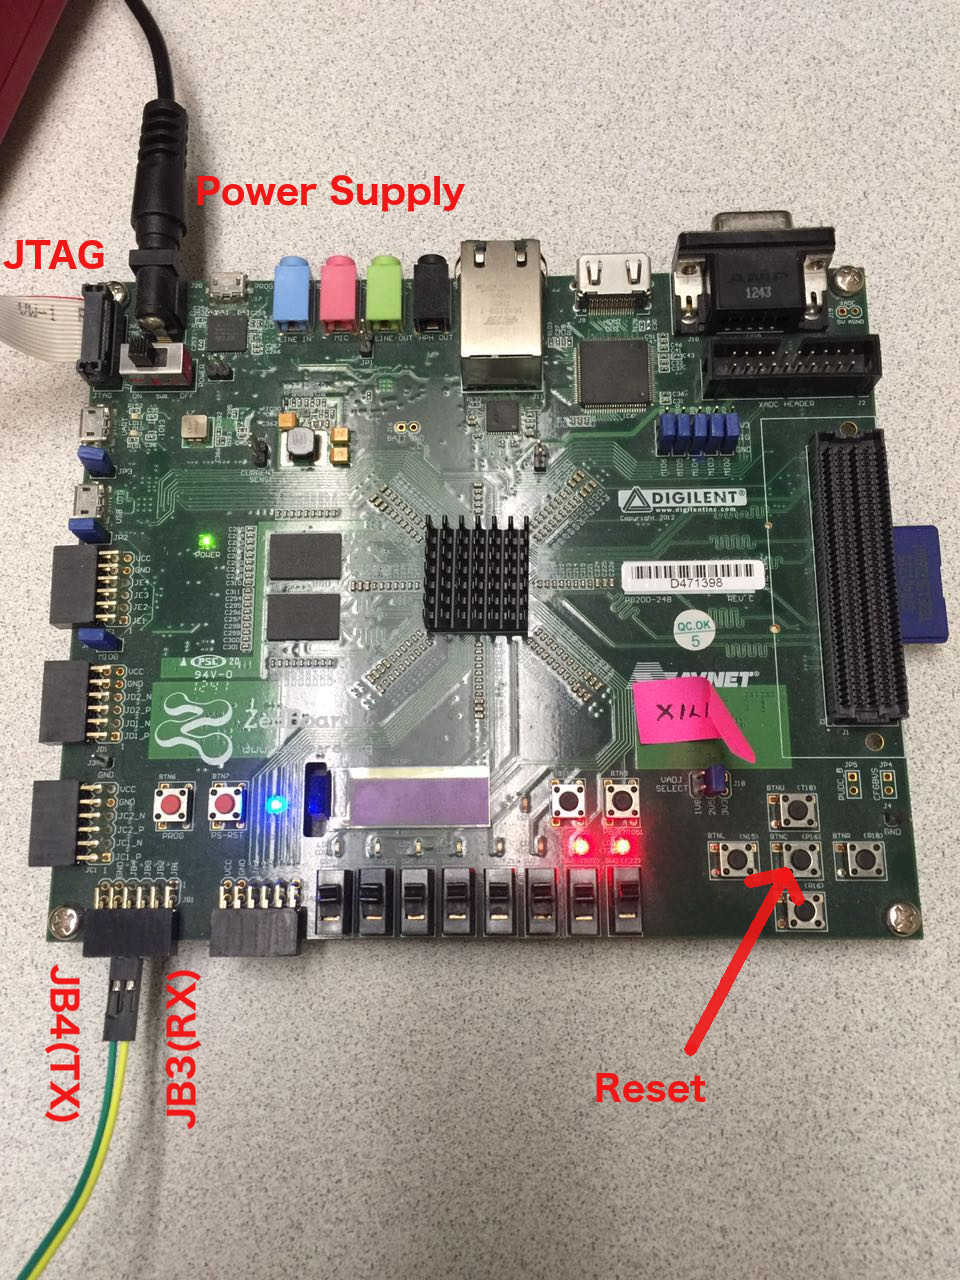
\includegraphics[width=8cm]{./fig/FPGA.jpg}
\centering
\end{figure}

\begin{figure}[h]
\caption{UART module connection setup}
\label{uart}
\includegraphics[width=8cm]{./fig/UART.jpg}
\centering
\end{figure}

\clearpage

% \subsubsection{Run on R2 FPGA}
% We fetched absolute position sensor (APS) data in the hardware. There are two APSs: APS1 and APS2. Each APS is stored in a 19bit raw data format. Figure.\ref{aps} show the relationship of raw APS data value and the real radius.\\
% In our design, we configured the at\_checker.vhd to sum up APS1 and APS2. In this way, the sum will keep around a constant value (e.g. x0\_0050). When we apply torque on the joint, the sum will shift based on the torque. The shift should within a reasonable range. In Figure.\ref{aps} (c), the red line is the sum with 0 torque applied. The green area is the reasonable shift range we defined. The task of the R2U2 is to measure whether the sum is in the green area or not.
% \begin{figure}[h]
% \caption{Signal Graph of APS1, APS2 and the Combination}
% \label{aps}
% 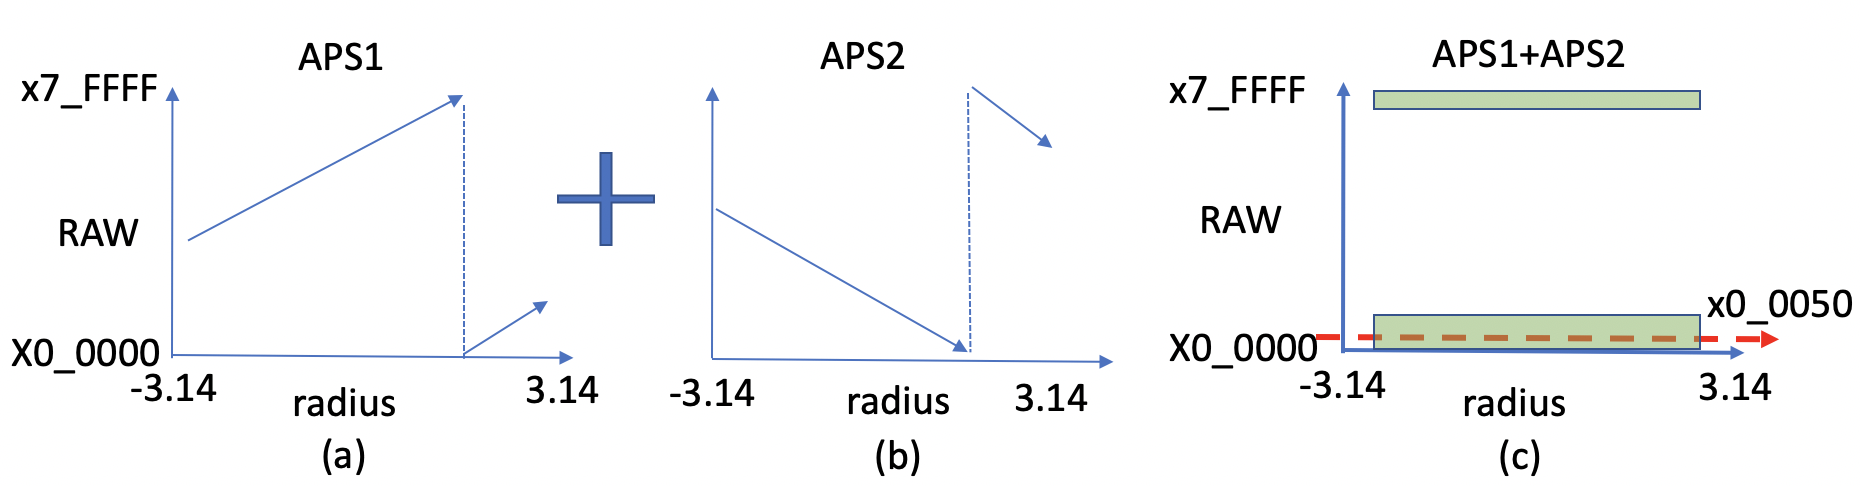
\includegraphics[width=16cm]{./fig/APS.png}
% \centering
% \end{figure}




% \subsection{Workflow}
% \begin{figure}[h]
% \caption{Demo Workflow}
% \label{workflow}
% 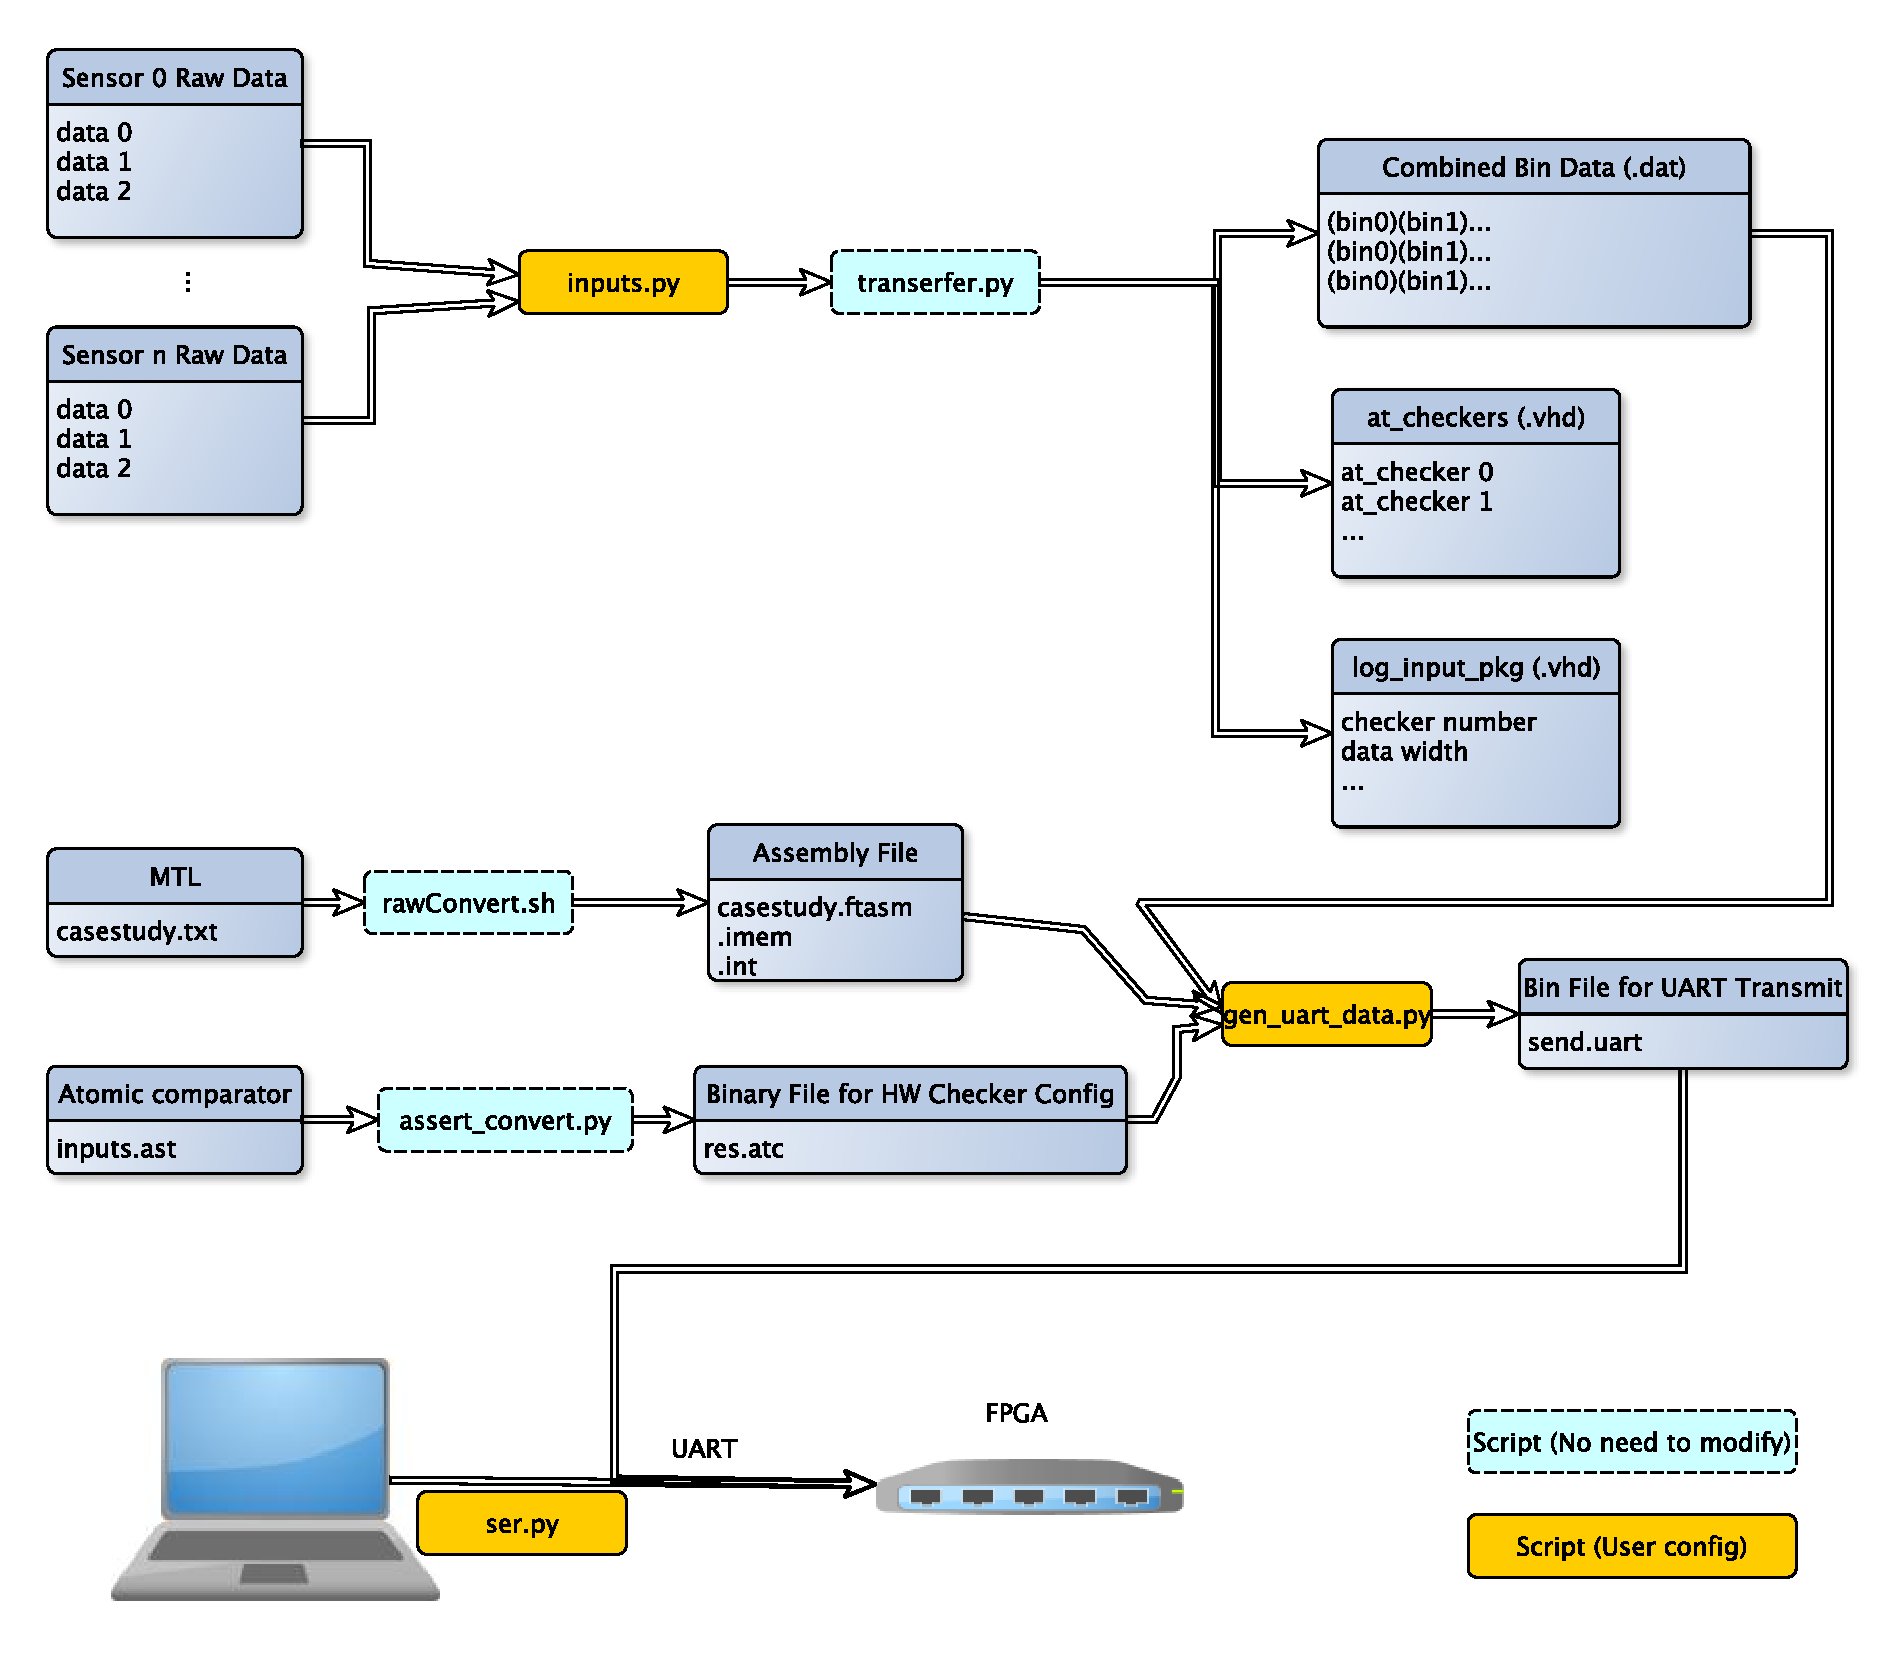
\includegraphics[width=15cm]{./fig/r2u2_process.eps}
% \centering
% \end{figure}

% \clearpage

% \subsection{Design Structure}
% \begin{figure}[h]
% \caption{Structure of R2U2 Hardware Component}
% \label{workflow}
% 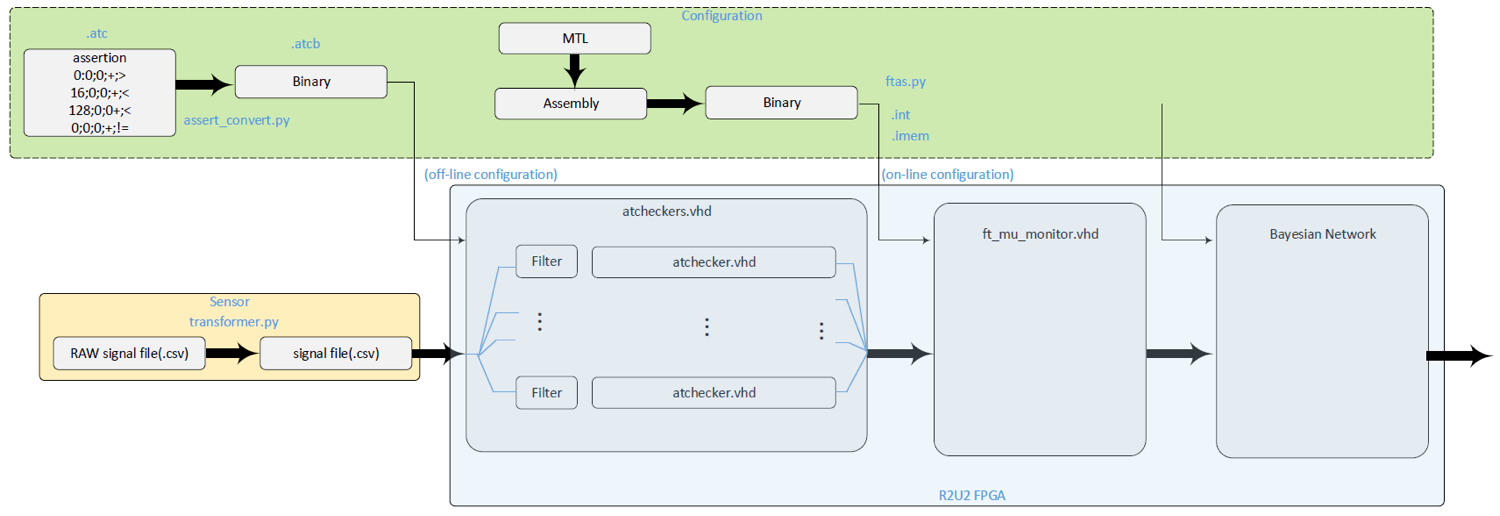
\includegraphics[width=16cm]{./fig/project_structure.png}
% \centering
% \end{figure}

\clearpage





\appendix
\section{\\File Structure}
\begin{forest}
  for tree={
    font=\ttfamily,
    grow'=0,
    child anchor=west,
    parent anchor=south,
    anchor=west,
    calign=first,
    inner xsep=7pt,
    edge path={
      \noexpand\path [draw, \forestoption{edge}]
      (!u.south west) +(7.5pt,0) |- (.child anchor) pic {folder} \forestoption{edge label};
    },
    before typesetting nodes={
      if n=1
        {insert before={[,phantom]}}
        {}
    },
    fit=band,
    before computing xy={l=15pt},
  }
[scripts/
  [config.py (setup all the configuration parameters in this file)
  ]
  [at\_checker/(generate VHDL file for atomic checker)
    [inputs.py(list all the atomic checkers and signals width here)
    ]
  ]
	[ftAssembler/
		[casestudy.txt (write the MTL formula here)
		]
		[rawConvert.sh (script to compile MTL into assemply)
		]
		[compiler/
		]
	]
  [sensor\_data.dat (write the sensor data here for simulation purpose)
  ]
	[gen\_log\_data.py (convert the sensor\_data.dat into binary format)
	]
	]
	[inputs.ast (configure each atomic checker)
	]
	[assert\_convert.py (convert inputs.ast into binary format)
	]
	[gen\_uart\_data.py (convert all the binary configuration file into Byte, which will send through UART)
	]
  [ser.py (python script to configure FPGA and read result through UART)
  ]
]
\end{forest}



\section{\\Details of Scripts and Files}
\subsection{inputs.py}\label{inputs.py}
(only compatiable with python 2.x)\\
Processing raw data file (similar to .csv) to the data format we want.\\
Parameters and functions:
\begin{enumerate}
	\item DATA\_SET: Raw data set file
	\item class subclass(CsvParser): \\
e.g.
\begin{lstlisting}[language=Python]
class Gs111m(CsvParser):
	def __init__(self):
		CsvParser.__init__(self)
		self.file = DATA_SET + "/gs111m_0.csv"
		self.addConfig(9, "float", 10, 24, "roll_angle", "in 1/2^10 rad")
		self.addConfig(8, "float", 10, 24, "pitch_angle", "in 1/2^10 rad")
\end{lstlisting}
Comment: Create a subclass. It will subtract the data you mentioned in \textbf{self.addConfig} and output the processed data into \textbf{self.file}
The self.file will look like:
\begin{center}
\begin{tabular}{ c|c}
 \hline
 roll\_angle & pitch\_angle \\
 \hline
 -42 & 12 \\
 \hline
 -34 & 6\\
 \hline
 -25 & 3\\
 ...&...
\end{tabular}
\end{center}
$\triangleright$ self.addConfig(channel, type, comma, width, name, comment)\\
@ channel: Column of the data in the raw data file.\\
@ type: Float or not. If it's float, write "float", else leave null.\\
@ comma: Only used for floating data type. It specifies how many fraction bit in binary you want to reserve during the conversion.\\
@ width: Number of bits for this data.\\
@ name: Specify the name of the column data. This will affect the name used in the .vhd code.\\
@ comment: Add any comment in string as you want.

\item class subclass(AtChecker):\\
e.g.
\begin{lstlisting}[language=Python]
class AtCheckerConfig(AtChecker):
	def __init__(self, inputFiles):
		AtChecker.__init__(self, inputFiles)
		self.add("pitch_angle", "", 1, "", "", "", "")
		self.add("roll_angle", "", 1, "", "", "", "")
\end{lstlisting}
Comment: Create a subclass. The subclass specifies the filters, number of atomic checkers, etc.. The class will affect at\_checker.vhd\\
$\triangleright$ self.add(input1, input2, count, filter1, filter2, rate1, rate2)\\
@ input1: First input to the at\_checker\\
@ input2: Second input to the at\_checker, usually used for compare with @input1. We can leave it as a null string "".\\
@ count: How many atomic checkers you want for this signal.\\
@ filter1: Hardware filter you want to use for input1. The filter name should be the same as the hardware filter component\\
@ filter2: Hardware filter you want to use for input2.\\
@ rate1: Signal delta during each sampling clk for input1. Leave null if you want to monitor signal delta.\\
@ rate2: Signal delta during each sampling clk for input2.

\end{enumerate}


\subsection{input.ast}\label{input.ast}
Atomic assertion file. Specify the at\_checker.vhd operation mode. For details, refer to \textbf{Performance\_Aware\_Hardware\_Runtime\_Monitors.pdf}.
\\
e.g.\\
\begin{tabular}{|p{0.98\textwidth}|}
\hline
-16;0;0;+;$>$\\
1;0;0;+;$=$\\
100;0;0;+;$>$\\
\hline
\end{tabular}
\\
\begin{figure}[h]
\caption{Atomic checker block}
\label{ac}
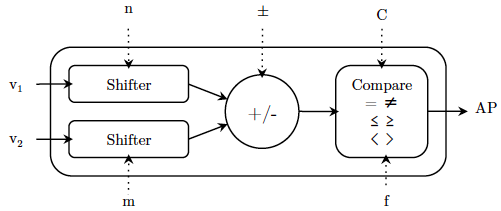
\includegraphics[width=8cm]{./fig/ast.png}
\centering
\end{figure}
Each line specifies the configuration for one atomic checker block. Consider the structure
of an atomic checker, depicted in Figure.\ref{ac}, then each line in the configuration file reads as:
C;n;m;+/-;f.

\subsection{gen\_uart\_data.py}\label{gendata.py}
Generate uart data byte by byte. Requires \textbf{.atc}, \textbf{.imem}, \textbf{.int} and \textbf{.dat} as input. I suggest leave the \textbf{.dat} file empty for the demo purpose.\\
%\begin{enumerate}
%	\item
%	\item class subclass(CsvParser): \\
%\end{enumerate}
Parameters:\\
@ SETUP\_DATA\_WIDTH\_extend\_byte: \textbf{.atc} file configuration data width.\\
@ SETUP\_ADDR\_WIDTH\_extend\_byte: \textbf{.atc} file configuration address width.\\
@ DATA\_BYTE\_WIDTH\_extend\_byte: binary logged data bit width (each line width of \textcolor{purple!30}{logged\_data.dat}).\\
These three parameters should be the same as in \textcolor{purple!30}{R2U2\_pkg.vhd}.

 \subsection{ser.py}\label{ser.py}

 \begin{enumerate}
 	\item serial.Serial()\\
	e.g.
	\begin{lstlisting}[language=Python]
ser = serial.Serial(
    port='/dev/ttyUSB0',
    timeout=0,
    # baudrate=9600,
    # parity=serial.PARITY_ODD,
    # stopbits=serial.STOPBITS_TWO,
    # bytesize=serial.SEVENBITS
 )
	\end{lstlisting}

Comment: By default, it is 9600 baud rate 8IN1 mode. You only need to specify the PC port that the UART is connecting to.
	\item parameters:
	@ DATA\_BYTE\_WIDTH\_extend\_byte: (same as \textcolor{purple!30}{gen\_uart\_data.py})
  \end{enumerate}

\end{document}

\clearpage

\end{document}
